\scanpage{101}

\deleted{Posons $q''=4q'=-4q$, $\omega''=8\omega$, de sorte que}

\[
\begin{aligned}&\deleted{\delta(q'')=-2^6\delta(q)=2^6\omega^{\otimes2}=(8\omega)^{\otimes2}=\omega''^{\otimes2}}\\&\deleted{\delta(q'')=\omega^{\unsure{\prime\prime}\otimes2}}\end{aligned}
\]

\deleted{La formule (\unsure{15|11|25}) prend la forme}

\[
\deleted{q''(}\tag*{(26)}
\]

\uline{Remarque} Posons

\[
q_\lambda=\lambda q\qquad\varphi_\lambda=\lambda\varphi\qquad [\,,\,]_{\lambda,\mu}=\deleted{\unsure{\tfrac1{\lambda}}}\inserted{(\lambda\mu)^{-1}}[\,,\,],\quad\omega_\mu=\mu\omega
\]

\deleted{La formule (8) s'écrit alors}

\[
\deleted{q_\lambda([x,y]_\lambda)=\lambda}
\]

\[
\deleted{2x\wedge y\wedge z=\varphi_\lambda([x,y]_\lambda,z)\,\omega}
\]

donc on a

\[
\left\{\begin{aligned}&\underline{\delta'(q_\lambda)}\bigl[=\lambda^3\delta(q)=-\underline{\lambda^3}\omega^{\otimes2}\bigr]=\underline{-\lambda^3\mu^{-2}\omega_\mu^{\otimes2}}\\ &\underline{2x\wedge y\wedge z}=\underline{\varphi_\lambda([x,y]_\lambda,z)\,\omega_\mu^{\unsure{3}}}\end{aligned}\right.
\]

\[
\left\{\begin{aligned}q_\lambda([x,y]_{\lambda,\mu})&=\lambda(\lambda\mu)^{-2}q([x,y])=-4\lambda^{-1}\mu^{-2}q(x)q(y)\sin^2(\widehat{x,y})\\ &=-4\lambda^{-3}\mu^{-2}q_\lambda(x)q_\lambda(y)\sin^2(\widehat{x,y})\end{aligned}\right.
\]

On veut choisir $\lambda,\mu$ tels que $-4\lambda^{-3}\mu^{-2}=1$ i.e. $\lambda^{-3}\mu^{-2}=-\frac14$ avec $\lambda,\mu$ des \inserted{(au signe près)} puiss. de 2

\figure{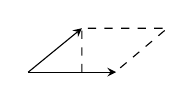
\begin{tikzpicture}[scale=.62,>=stealth]\draw[->] (0,0)--(1.8,0);\draw[->] (0,0)--(1.1,.9);\draw[dashed] (1.1,0)--(1.1,.9)--(2.85,.9)--(1.78,0);\end{tikzpicture}}

\[
\lambda=-2^\alpha,\ \mu=2^\beta\qquad \lambda^{-3}\mu^{-2}=-2^{-(3\alpha+2\beta)}=-2^2
\]

i.e. on veut $3\alpha+2\beta=-2$ p.ex. on prend $\alpha=0$, $\beta=\deleted{\unsure{0|-}}1$ ce qui donne

\[
\lambda=-1,\ \mu=1/2\qquad q_\lambda=\inserted{q'\deleted{\unsure{_\lambda}}}=-q,\quad\omega_\mu=\unsure{2|1}\omega'=\tfrac12\omega
\]

\inserted{$[x,y]_{\lambda,\mu}=[x,y]'=-2[x,y]$}

\[
\left\{\begin{aligned}\delta'(q')&=+4\omega'^{\otimes2}=(2\omega')^{\otimes2}\\ x\wedge y\wedge z&=\tfrac12\varphi'([x,y]',z)\,\omega'\\ q'([x,y]')&=q'(x)q'(y)\sin^2(\widehat{x,y})\\ &=q'(x)q'(x)\bigl(1-\tfrac14\varphi(x,y)^{2}\bigr)\end{aligned}\right.
\]

% archive sheet number: 100
